\documentclass[12pt,a4paper]{article}
\usepackage[polish]{babel}
\usepackage[T1]{fontenc}
\usepackage{lmodern}
\usepackage[utf8x]{inputenc}
\usepackage{hyperref}
\usepackage{url}
\usepackage{graphicx}
\usepackage{listings}
\title{Landscape Generator\\Inżyniera Oprogramowania}
\author{Artur Bednarczyk, Dawid Grajewski, Tomasz Januszek\\Politechnika Śląska\\Wydział Matematyki Stosowanej\\Informatyka, semestr IV}
\date{\today}

\begin{document}
\maketitle
\newpage
\tableofcontents
\newpage
\section{O projekcie}
\subsection{Zespół}
Artur Bednarczyk, Dawid Grajewski, Tomasz Januszek.
\subsection{Temat}
TREŚĆ ZADANIA
\subsection{Cel}
Opis treści.
\section{Projekt}
\subsection{Plany i pomysły}
Co chcemy zrobić
\subsection{UI/UX}
\subsubsection{Zawartość}
\subsubsection{Projekty UI}
\section{Teoria}
\subsection{Losowość}
Kilka słów o losowości w naszej aplikacji.
\subsection{Algorytmy}
\subsubsection{Szum Perlina}
Szum Perlina - co to jest, opis algorytmu itp.
\section{Narzędzia}
\subsection{Kontrola wersji}
Do zarządzania kodem i wersjami projektu wykorzystujemy narzędzie Git. Korzystamy z platformy GitHub jako repozytorium dostępnego online. Dobór narzędzi służących do korzystania z repozytorium to sprawa indywidualna każdego członka zespołu, ponieważ nie ma ona wpływu na sam projekt.
\subsection{Zarzadzanie zespołem}
Trello - Kanban Board
\subsection{Środowisko}
Visual Studio
\section{Aplikacja}
\subsection{Architektura}
Wzorce architektoniczne
\subsection{Struktury danych}
Dane przechowujemy ...
\subsection{Schemat graficzny struktury systemu}
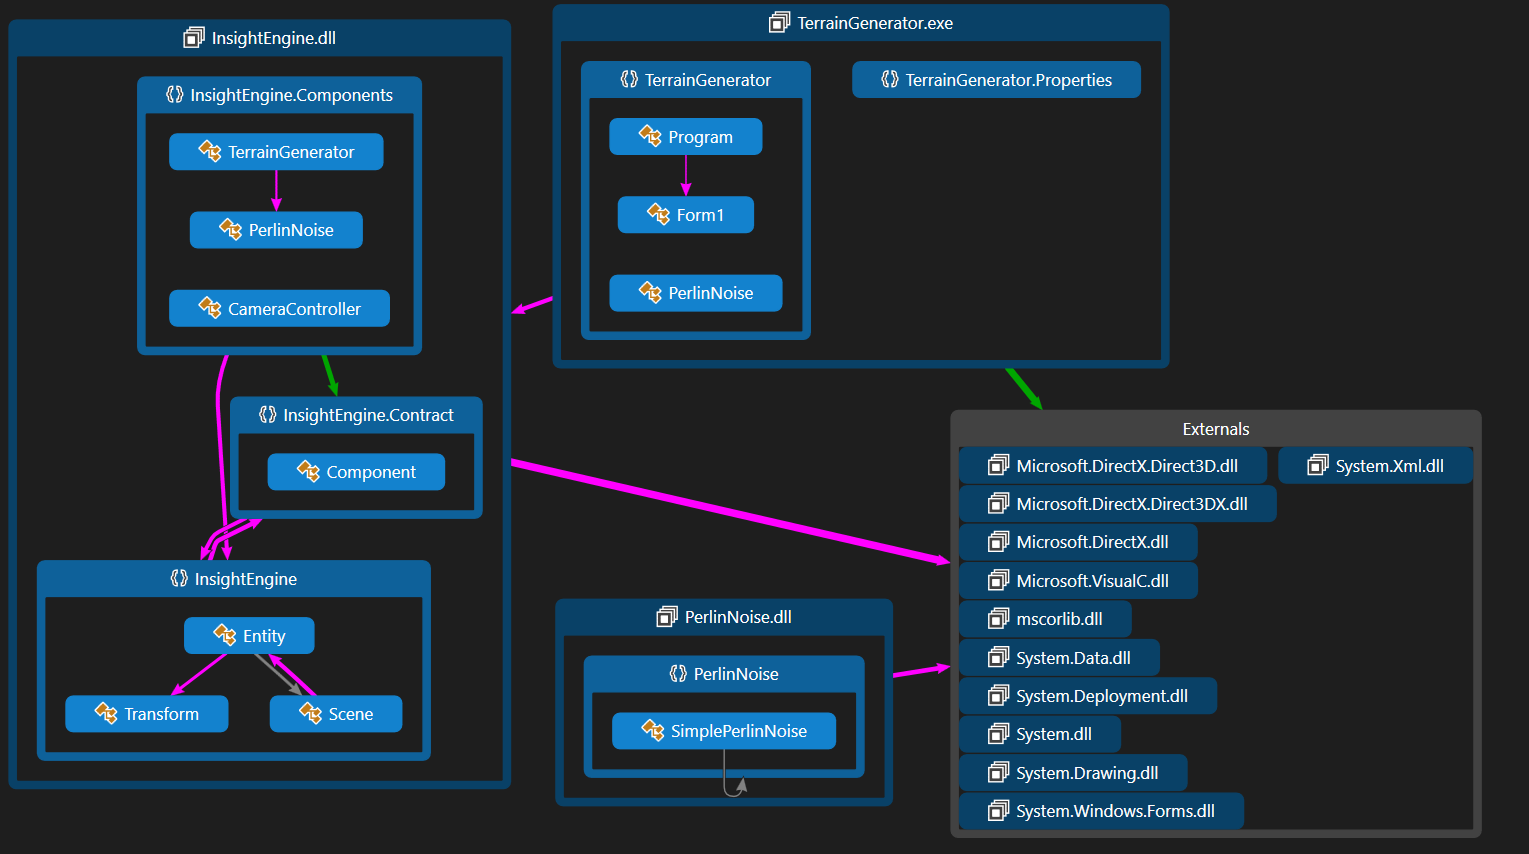
\includegraphics[width=1\textwidth]{images/klasy.png}
\subsection{Komunikacja między modułami}
Jak to wszystko się komunikuje
\section{API}
\subsection{Perlin}
Tworzymy obiekt PerlinNoise, który wymaga podania rozmiaru i wymiarów.
\end{document}